\documentclass[10pt]{beamer}
\usepackage[utf8]{inputenc}
\usepackage[T1]{fontenc}
\usepackage{lmodern}
\usetheme{Cuerna}
\usepackage{hyperref}
\usepackage[spanish]{babel}
\usepackage{multicol}
\usepackage{graphicx}
\title{Análisis de Productos}
\author{Angélica María Martínez Céspedes}
\date{20 de julio del 2023}



    \title{{\Huge \textbf{\textit{Análisis de Productos}}}}
    \author{Angélica María Martínez Céspedes}
    \date{\textbf{20 de julio del 2023}}
    \subtitle{CERVEZA CEBOLLA REFRESCO}
    \institute{\textbf{{\scriptsize Facultad de Matemática y Computación}}}
   
  
\begin{document}
   	\begin{frame}
   		\titlepage
   	\end{frame}
   	
   
   	
  
   	\begin{frame}
   		
   		\begin{center}
   			{\LARGE{\textbf{\textit{Cerveza  Cebolla  Refresco}}}}
   		\end{center}
   		
   		\begin{figure}
   			\centering
   			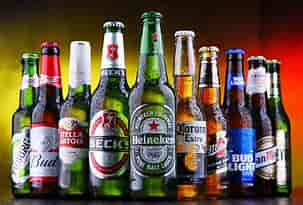
\includegraphics[width=0.2\linewidth]{FIGURA/cervezas}
   			\caption{}
   			\label{fig:cervezas}
   		\end{figure}
   		
   	
   	   \begin{figure}
   	   	\centering
   	   	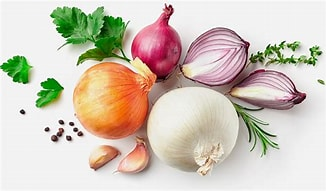
\includegraphics[width=0.2\linewidth]{FIGURA/cebolla}
   	   	\caption{}
   	   	\label{fig:cebolla}
   	   \end{figure}
   	   
   	
   	  
   	  \begin{figure}
   	  	\centering
   	  	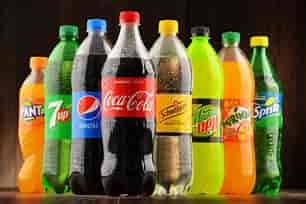
\includegraphics[width=0.2\linewidth]{FIGURA/refrescos}
   	  	\caption{}
   	  	\label{fig:refrescos}
   	  \end{figure}
   	  
   	   
   	\end{frame}
   	
   	 	
   	\begin{frame}{\textbf{\textit{Introducción}}}
   	 \begin{center}
   			Se analizaron los datos de los productos:cerveza,cebolla y refresco en el municipio del Cerro,donde se estudiaron los precios de cada uno de estos productos,su promedio,el precio más común,marcas y tipos que más predomina de cada uno de ellos,además de otros aspectos significativos.
   	 \end{center}
   	\end{frame}
   	
   	\begin{frame}{\textbf{\textit{Desarrollo}}}
   		
   		A continuación se presentará en cada una de las diapositivas el desarrollo de la realizada investigación sobre los productos antes mencionados,además de las conclusiones llevadas a cabo luego de cada análisis con el apoyo de gráficos para obtener una mejor visualización de los datos. 
   	
   	       
   	
   	\end{frame}	
   		
   	
   	\begin{frame}{\textbf{\textit{Análisis de la Cerveza}}}
   		
   	   La cerveza tiene una variación de precios bastante amplia desde su precio mínimo que en este caso es \$125 hasta su precio máximo que es \$300 , ambos reflejados claramente en el gráfico anterior, el cual no se encuentra ordenado de mayor a menor pero sí , se puede compreder debido a que el tamaño de cada barrita informa su precio , que distingues mejor por la escala , además el precio más común de la cerveza es 150 , personalizado con la raya roja en línea vertical que se puede observar , esta información es de gran utilidad para los consumidores puesto que si un cliente tiene conocimiento del precio máximo , mínimo y más común del producto que quiere consumir , puede tomar decisiones informadas sobre cuánto está dispuesto a pagar por una cerveza en particular o por un producto en si.
   	   
   	\end{frame}
   	
   	\begin{frame}
   		
   	\begin{figure}
   		\centering
   		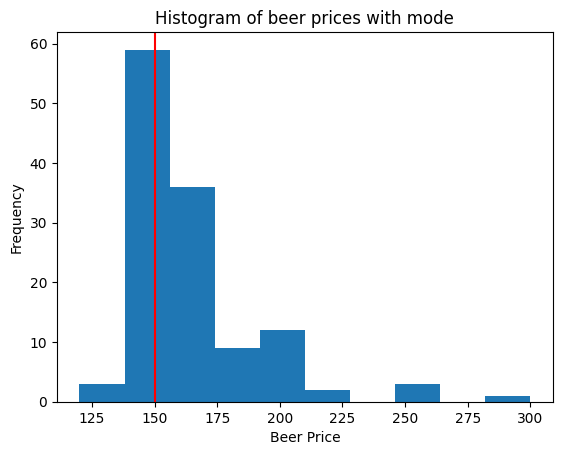
\includegraphics[width=0.7\linewidth]{FIGURA/gráfico precios cerveza}
   		\caption{}
   		\label{fig:grafico-precios-cerveza}
   	\end{figure}
   	
   	\end{frame}
   	
    
    \begin{frame}
    	
     Es de gran utilidad tener el conocimiento sobre los píses de origen de las cervezas que más predominan en el ayuntamiento , pues se llega a la conclusión precisa de que la mayoría de estas cervezas son importadas donde destacan Bélgica , Holanda y España como los tres países con mayor \% , lo que significa que son los países que más importan las cervezas que predominan en el municipio del Cerro.
    	
    \end{frame}
   	
   	\begin{figure}
   		\centering
   		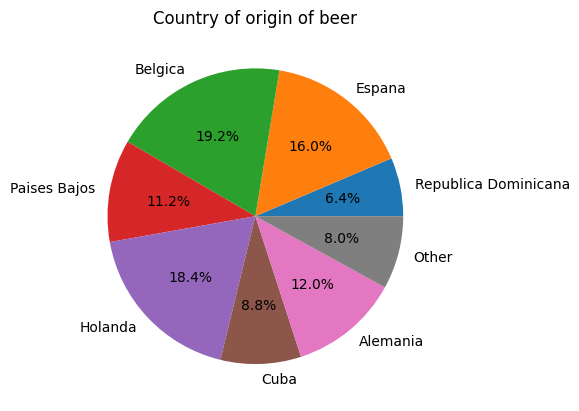
\includegraphics[width=0.7\linewidth]{FIGURA/países de origen}
   		\caption{Países de procedencia}
   		\label{fig:paises-de-origen}
   	\end{figure}
   	
   	
   	\begin{frame}
   		
   	    Los precios promedios de cada marca de cerveza , donde la cerveza más cara es la Patronus que tiene un costo de 250\$ y la más económica es la Cruz Campo con un precio de 130\$ apróximadamente.La relación entre la marca de la cerveza y su precio aporta información valiosa sobre la demanda y la asequibilidad del producto , no obstante que una cerveza tenga un precio más bajo que otra no quiere decir que tenga una demanda mayor , simplemente puede deberse a que tiene menor distinción de marca , en este caso que la cerveza Cruz Campo o cualquiera de las cervezas importadas representadas en el segundo gráfico tengan un precio más económico que las cervezas del primer gráfico no quiere decir que sean más populares ni tenga mayor credibilidad que las demás , puesto que la Patronus , cerveza procedente de Alemania la cual como se reveló con anterioridad cuesta 250\$ y este país es considerando el cuarto mayor exportador de cerveza otorgándole distinción y credibilidad a sus productos , también se destaca Holanda que importa la Hollandia Premium y la Holland Import que ambas tienen un precio que oscila entre 150-200\$ y tienen alta demanda y credibilidad en el mercado . 
   	    
   	\end{frame}
   	
   	
   	\begin{frame}
   	
   	\begin{figure}
   		\centering
   		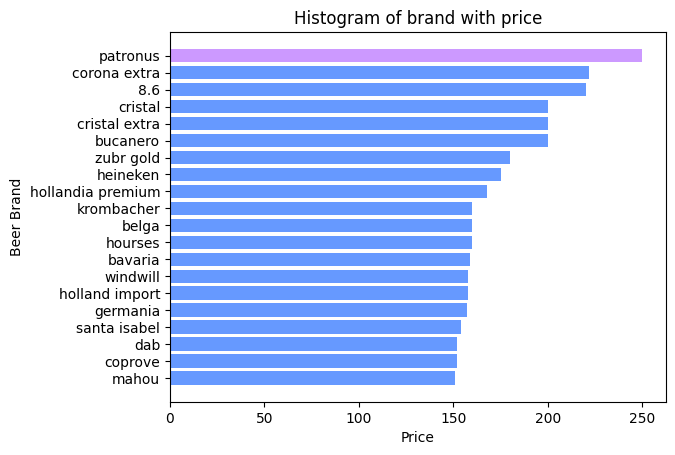
\includegraphics[width=0.4\linewidth]{FIGURA/precios promedios}
   		\caption{Mayores Precios Promedios}
   		\label{fig:precios-promedios}
   	\end{figure}
   	
   	\begin{figure}
   		\centering
   		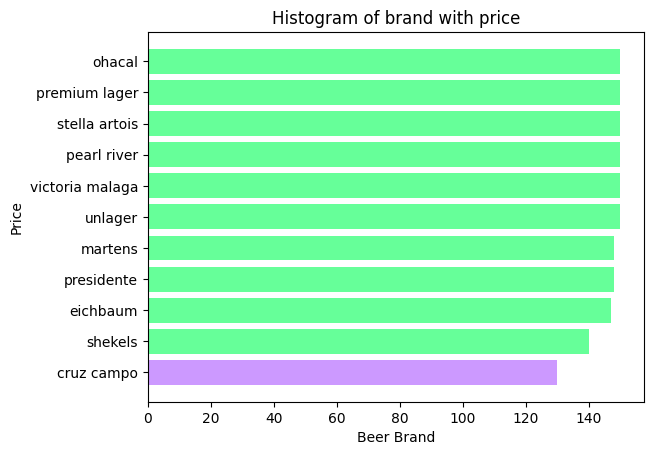
\includegraphics[width=0.4\linewidth]{FIGURA/precios promedios menores}
   		\caption{Menores Precios Promedios}
   		\label{fig:precios-promedios-menores}
   	\end{figure}
   	
   	\end{frame}
   	
   	\begin{frame}
   		La cantidad de ml de una lata o botella de cerveza parece un aspecto insignificante , sin embargo es todo lo contrario , si se tiene en cuenta el precio de cada marca de cerveza , dato importante que se presento en observaciones anteriores , cuando comparas cada precio de esa cerveza con su cantidad de ml te podrás dar cuenta de que la cerveza más económica no es la opción más factible en todas los casos , pues puede que tenga menor cantidad de ml.
   		
   		\begin{figure}
   			\centering
   			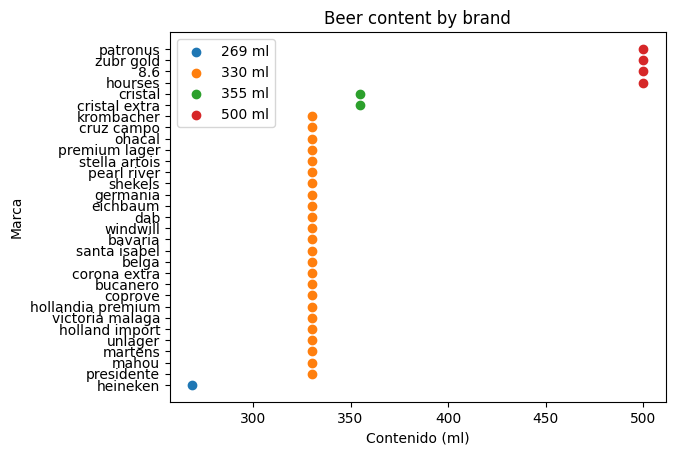
\includegraphics[width=0.4\linewidth]{FIGURA/cantidad ml}
   			\caption{Cantidad de ml de cada marca de cerveza}
   			\label{fig:cantidad-ml}
   		\end{figure}
   		
   	\end{frame}
   	
   	
   	\begin{frame}
   		El porcentaje de alcohol de la cerveza es una medida de la cantidad de etanol que contiene,además este porciento puede variar en dependencia según el país de procedencia , por ejemplo en algunos países europeos como Bélgica y Alemania , es común encontrar cervezas con mayor \% de alcohol, mientras que en otros países como en Estados Unidos , las cervezas suelen tener un porcentaje de alcohol más bajo.Este \% también puede estar relacionado con la tradición cervecera del país de origen y los ingredientes utilizados para elaborarl.La cerveza con mayor \% de alcohol,en este caso es la 8.6 que curiosamente su nombre coincide con su \% de alcohol.
   		
   		\begin{figure}
   			\centering
   			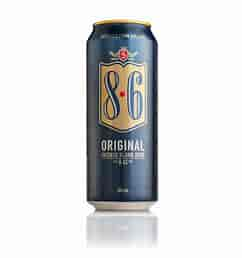
\includegraphics[width=0.3\linewidth]{FIGURA/8.6}
   			\caption{Cerveza con mayor \% de alcohol}
   			\label{fig:8}
   		\end{figure}
   		
   	\end{frame}
   	
   	
   	\begin{frame}
   		
   		\begin{itemize}
   			\item{Predomina el envase de \textit{\underline{lata}} sobre el de \textit{\underline{botella}}}
   		\end{itemize}
   		
   		\begin{figure}
   			\centering
   			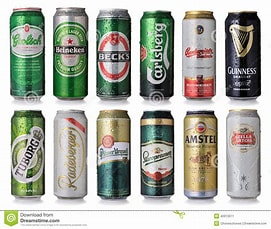
\includegraphics[width=0.2\linewidth]{FIGURA/latas}
   			\caption{Latas}
   			\label{fig:latas}
   		\end{figure}
   		
   		
   		\begin{figure}
   			\centering
   			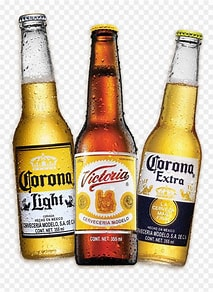
\includegraphics[width=0.2\linewidth]{FIGURA/botellas}
   			\caption{Botellas}
   			\label{fig:botellas}
   		\end{figure}
   		
   		
   	\end{frame}
   	
   	
   	\begin{frame}{\textit{Análisis de la Cebolla}}
   		
   		\begin{itemize}
   			\item{ Los precios promedios entre:}
   		\end{itemize}
   		
   		
   		\begin{enumerate}
   			\item {la cebolla blanca}
   			\item{la cebolla morada}
   		\end{enumerate}
   	  
   	  
   	  \begin{figure}[h]
   	  	\centering
   	  	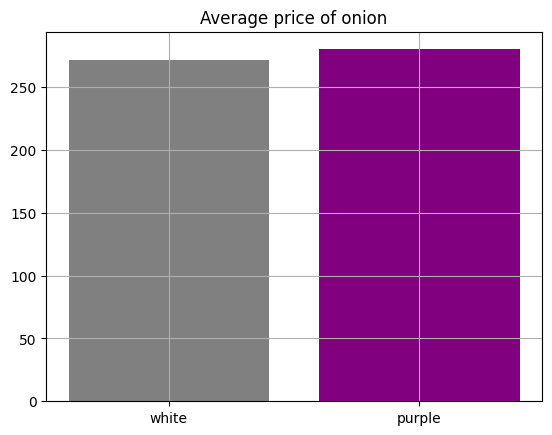
\includegraphics[width=0.4\linewidth]{FIGURA/precio promedio cebolla blanca y morada}
   	  	\caption{Promedios}
   	  	\label{fig:precio-promedio-cebolla-blanca-y-morada}
   	  \end{figure}
   	  
  	\end{frame}
   	
   	
   	\begin{frame}
   		 \begin{itemize}
   			\item{El precio más común entre ambas:}
   		\end{itemize}
   		
   		\begin{figure}
   			\centering
   			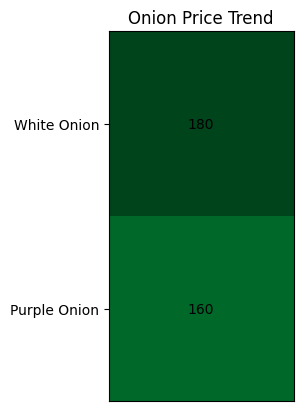
\includegraphics[width=0.4\linewidth]{FIGURA/moda cebolla}
   			\caption{Precio Moda}
   			\label{fig:moda-cebolla}
   		\end{figure}
   \end{frame}		
   		
   	\begin{frame}
   		
   		Predomina la venta de cebolla en libra,más que en ristra.
   		Además prevalece la venta de cebolla en agros,representado en el gráfico de pastel donde el color azul muestra la cantidad de agros,el naranja los carretilleros y el  verde un puesto en una casa, también en el próximo análisis quedará claro que realmente en el municipio  Cerro se puede encontrar tanto escazes de carretilleros como de agros.
   		
   		\begin{figure}
   			\centering
   			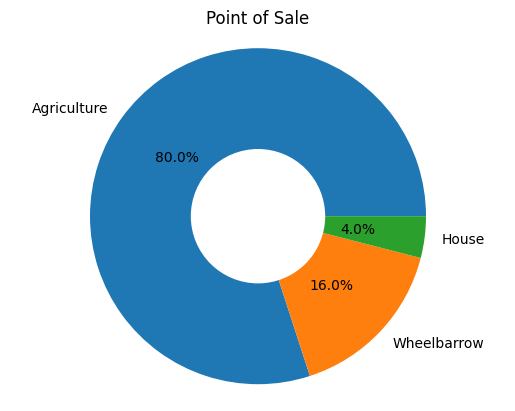
\includegraphics[width=0.4\linewidth]{FIGURA/puestos de venta cebolla}
   			\caption{Puestos de ventas}
   			\label{fig:puestos-de-venta-cebolla}
   		\end{figure}
   		
   	\end{frame}
   		
   	\begin{frame}
   		
   		
   		 El municipio Cerro es uno de los municipios más pequeños de la provincia de La Habana.Está postura puede conllevar a varias ventajas o desventajas como por ejemplo la concentración de áreas de consumo,esta situación logra ser de gran beneficio ya que se tienen todos los locales comerciales en el mismo sector ¿pero de ser el caso contrario que pasaría? 
   	
   		\begin{figure}
   			\centering
   			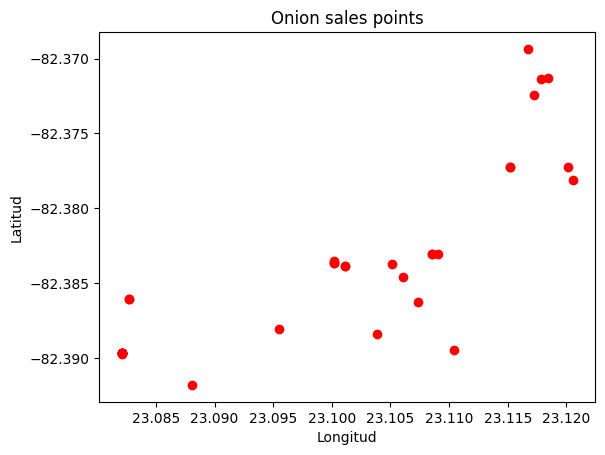
\includegraphics[width=0.3\linewidth]{FIGURA/grfdisperssión1}
   			\caption{venta cebolla}
   			\label{fig:grfdisperssion1}
   		\end{figure}
   		
   		\begin{figure}
   			\centering
   			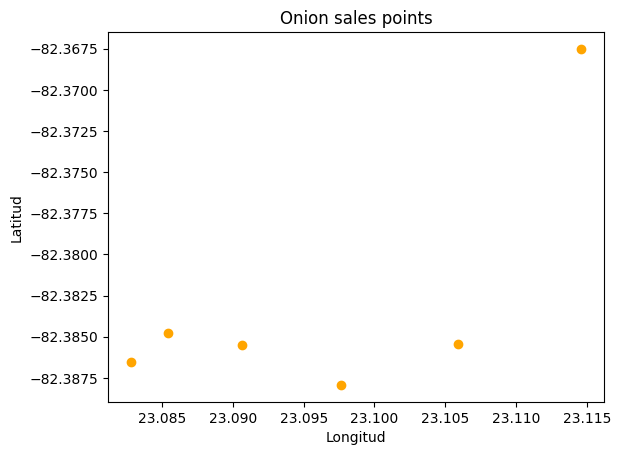
\includegraphics[width=0.3\linewidth]{FIGURA/grafdispersión2}
   			\caption{no hay cebolla}
   			\label{fig:grafdispersion2}
   		\end{figure}
   		
   		
   	\end{frame}	
   		
  
   	
   \begin{frame}{\textit{Análisis de los Refrescos}}
   	
   	Al analizar el precio promedio de cada marca de refresco y representarlos graficamente se observa una variedad de precios bastante amplia.
   	
   	  \begin{figure}
   		\centering
   		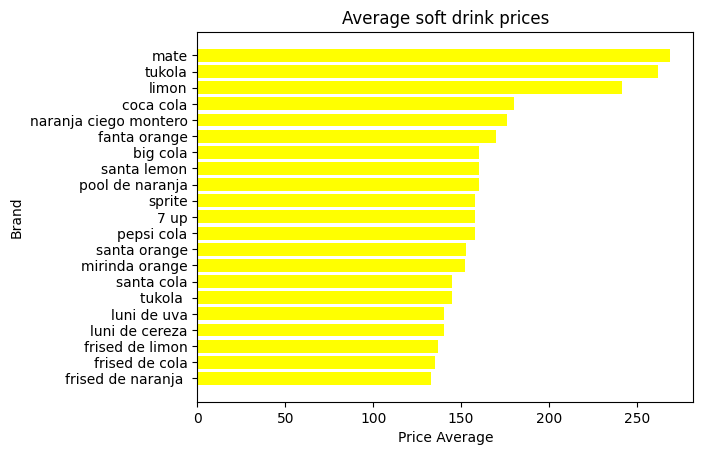
\includegraphics[width=0.6\linewidth]{FIGURA/promedios refrescos}
   		\caption{}
   		\label{fig:promedios-refrescos}
     \end{figure}
   	
   \end{frame}
   	
   	\begin{frame}
   		
   		\begin{itemize}
   			\item{El precio más común de los refrescos es \$150.}
   				\item{Los refrescos en\underline{ Lata} prevalecen más que los refrescos en \underline{Pomo.}}
   			\item{La marca de refrescos que más predomina es la \underline{Pepsi Cola}.}
   	    \end{itemize}
   		
   		
   		\begin{figure}
   			\centering
   			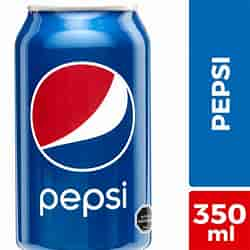
\includegraphics[width=0.3\linewidth]{FIGURA/pepsi cola}
   			\caption{}
   			\label{fig:pepsi-cola}
   		\end{figure}
   		
   	\end{frame}
   	
   	
   	\begin{frame}
   		
   		Cada producto contiene en la etiqueta de su envase la información sobre la cantidad de energía y nutrientes por 100  gramos o 100 mililitros del alimento,dicha información es obligatoria en el etiquetado nutricional,dicha información se considera indispensable.
   		
   		
   		\begin{figure}
   			\centering
   			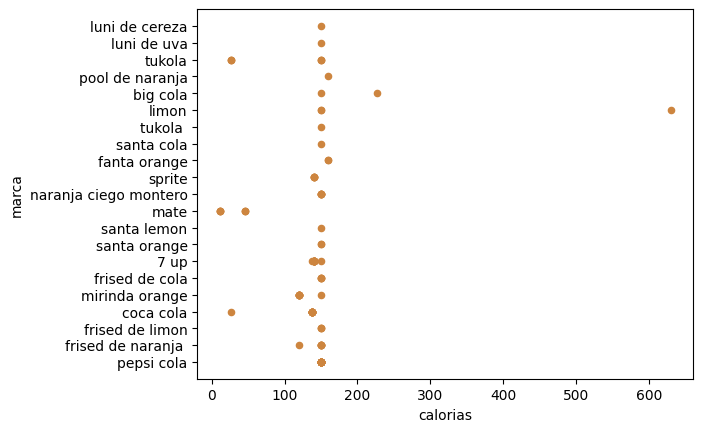
\includegraphics[width=0.6\linewidth]{FIGURA/calorías refrescos}
   			\caption{Calorías por 100 gramos}
   			\label{fig:calorias-refrescos}
   		\end{figure}
   		
   	\end{frame}
   	
   		
   	\begin{frame}
   		
   		El país que mayor cantidad de refrescos importa a Cuba es Estados Unidos,territorio donde nacieron dos de los máximos referentes de la industria mundial:
   		
   		\begin{enumerate}
   			\item{Pepsi-Cola}
   			\item{Coca-Cola}
   		\end{enumerate}
   		
   		\begin{figure}
   			\centering
   			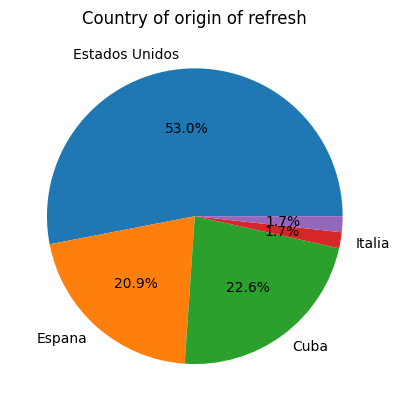
\includegraphics[width=0.5\linewidth]{FIGURA/países refrescos}
   			\caption{Países de procedencia de los refrescos}
   			\label{fig:paises-refrescos}
   		\end{figure}
   		
   	\end{frame}
   	
   	
   	\begin{frame}{\textbf{\textit{Conclusiones}}}
   		
   		Según los análisis realizados de cada producto,se concluye que hay factores comunes de cada producto que tienen gran utilidad,tener conocimientos acerca de:
   		
   		\begin{itemize}
   			\item{La variación del precio de cada uno de ellos.}
   			\item{El precio promedio.}
   			\item{El precio moda.}
   			\item{Las marcas.}
   			\item{ La cantidad de ml.}
   			\item{Los beneficios de cada tipo cebolla,entre otros aspectos significativos.}
   		\end{itemize}
   		
   		  Se concluye que la  mayoría de las cervezas y refrescos que predominan en el país son los importados,y que el precio de cada uno de ellos no tiene mucha relación con su demanda en el mercado,que algunos de los países de origen que exportan estas marcas coinciden y se llega al resultado de que tienen una pequeña relación,además la escasez de cebollas y agros presentes en el municipio es un tema delicado que deberían tratar de solucionar por necesidad,y en beneficio de la población.
   		
   	\end{frame}
   	
  
\end{document}